\documentclass[a4paper,11pt]{article}

% Identificação
\newcommand{\pbtitulo}{Octave}
\newcommand{\pbversao}{1.0}

\usepackage{../sty/tutorial}
\usepackage{wrapfig} % Imagens que se cruzam com texto

%----------------------------------------------------------------------
% Início do Documento
%----------------------------------------------------------------------
\begin{document}
	
	\maketitle % mostrar o título
	\thispagestyle{fancy} % habilitar o cabeçalho/rodapé das páginas
	
%--------------------------------------------------------------------------
% RESUMO DO ARTIGO
%--------------------------------------------------------------------------
\begin{abstract}
	% O primeiro caractere deve vir com \initial{}
	\initial{O}ctave \cite{octaveoficial}, é um sistema interativo completo para cálculos numéricos com colaboradores em todo o mundo. É uma alternativa \textit{Open Source} ao MATLAB. Disponível sob a \textbf{GPL} (Licença Pública Geral do GNU) possui ferramentas extensivas para a resolução de problemas lineares numéricos comuns de álgebra, cálculo de equações não-lineares, funções ordinárias, polinômios, integrais e integração numérica de equações diferenciais ordinárias e diferenciais-algébricas. Então não serve para o Cientista de Dados? Nesta desejo provar o contrário e mostrar que podemos utilizar o Octave como ferramenta de auxílio ao nosso trabalho.
\end{abstract}

%--------------------------------------------------------------------------
% CONTEÚDO DO ARTIGO
%--------------------------------------------------------------------------
\section{Parte inicial}
Foi escrito por \textbf{John W. Eaton} em 1988 com o objetivo de ser usado como referência para a apostila no curso "Projetos de Reatores Químicos" de \textit{James B. Rawlings}, da Universidade \textit{Wisconsin-Madison} e \textit{John G. Ekerdt} da Universidade do Texas. Ou seja, originalmente idealizado como uma ferramenta especializada na solução de problemas para reatores químicos.
\begin{figure}[H]
	\centering
	
\includegraphics[width=0.3\textwidth]{imagem/logo}
	\caption{Logo do Octave}
\end{figure}

\textbf{GNU/Octave} (nesta trataremos somente por \textbf{Octave}) atualmente é utilizado de modo bem mais amplo, tanto no meio acadêmico com em aplicações comerciais. Existe um relacionamento profundo deste com o \textbf{MATLAB} (de MATrix LABoratory)que combina um ambiente desktop para análise iterativa, processos de projeto e uma linguagem de programação para expressar matrizes diretamente. Porém por ser um software proprietário cuja licença tem um valor não acessível ao usuário comum, a comunidade GNU resolveu adotar um substituto com uma grande semelhança dos comandos do Matlab e por aceitar os arquivos de mesmo formato.

Octave é uma linguagem voltada para computação numérica. Porém sua interface de comandos está bem mais parecida com o RStudio, sendo possível plotar gráficos e ler bancos de dados, imagens ou mesmo interagir com o Arduino. A grande vantagem é a disponibilização de pacotes que são criados pela comunidade e amplia os recursos do Octave para diversas experiências. Pode ser utilizado também em modo script (textos de programação). 

\section{No Ambiente Octave}
Após realizar a instalação do Octave e executá-lo, temos a seguinte tela:
\begin{figure}[H]
	\centering
	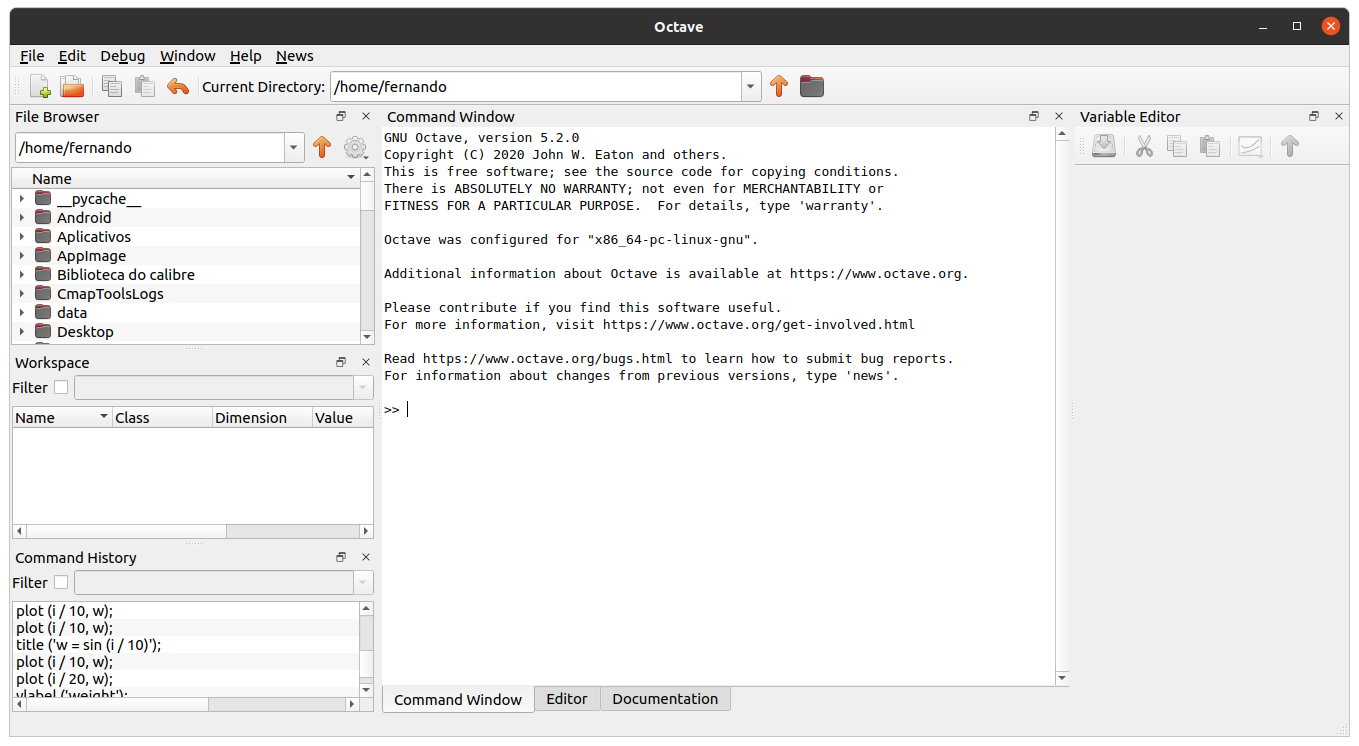
\includegraphics[width=0.8\textwidth]{imagem/ambiente}
	\caption{Ambiente do Octave}
\end{figure}

Bem parecido com o \textbf{RStudio}, na parte central se encontra a \textbf{Janela de Comandos} e é nesta que basicamente trabalhamos. Podemos obter um auxílio a qualquer comando: \\
\codigo{>> help comando}

Também existe a possibilidade de usar as setas para cima/baixo como forma de acessar os comandos já inseridos (é util quando desejamos repetir um comando). Começamos pelas operações matemáticas, digitar: \\
\codigo{>> 6 + 5}

E ao pressionarmos \opcbotao{ENTER } recebemos como resposta uma variável \textit{ans} com o valor 11. Na janela lateral a esquerda foi criada essa variável e a qualquer momento pode ser utilizada, digitar: \\
\codigo{>> ans * 2}

E agora \textit{ans} possui o valor 22, ou seja, cada operação matemática que realizamos alteramos o valor dessa variável que também pode ser utilizada em nossos cálculos. Além da adição ($+$), multiplicação ($*$), divisão ($/$) e subtração ($-$) também são permitidas operações primárias como divisão indireta ($\setminus$) que é realizada da direita para esquerda, ou seja, divisor é o primeiro elemento: \\
\codigo{>> 10 $\setminus$ 5}

Que é equivalente a: \\
\codigo{>> 5 / 10}

Também podemos usar a potencia ($\string^$): \\
\codigo{>> 10 $\string^$ 2}

Ou seja, 10 elevado a 2. Além da variável \textit{ans} que é criada e gerenciada automaticamente (outras são por exemplo: $pi$, $version$ ou $computer$). Podemos criar nossas variáveis através do comando de atribuição ($=$): \\
\codigo{>> a = 10 + 2 * 3}

Existem certas regras para nomear as variáveis. Os nomes devem ser iniciados por letras, não podem conter espaços nem caracteres de pontuação, diferença entre letras maiúsculas de minúsculas e alguns nomes são reservados. Na janela a esquerda aparece todas as variáveis criadas, neste caso \textbf{a} com o valor 16. Não deveria ser 36? É respeitado a precedência matemática dos operadores assim a multiplicação é realizada antes da adição. 

Com $;$ podemos agrupar comandos na mesma linha: \\
\codigo{>> a = 2; b = 4; a * b}

Temos a variável \textbf{a} com o valor 2, \textbf{b} com o valor 4 e \textbf{ans} com o valor 8. Listar todas as variáveis disponíveis: \\
\codigo{>> who}

\textbf{whos} lista além das variáveis informações adicionais sobre elas. Remover uma variável: \\
\codigo{>> clear a}

Ou todas as variáveis: \\
\codigo{>> clear all}

\begin{theo}[Limpar a Janela de Comandos]{}
	Digitar o comando: \codigo{clc} ou simplesmente pressionar $Ctrl+L$. Outros atalhos interessantes são $Ctrl+U$ limpa a linha atual ou $Ctrl+K$ limpa da posição do cursor para frente.
\end{theo}

\subsection{Formatação e precisão numérica}
Não existe a distinção entre valores inteiros ou decimais: \\
\codigo{>> a = 5.0; b = 5;}

Observamos que tanto a variável \textbf{a} quanto \textbf{b} possuem o mesmo valor \textbf{5}, e pertencem a mesma classe \textit{double}. Normalmente os números decimais são exibidos com quatro dígitos, se esses são significativos: \\
\codigo{>> a = 5.01234}

E agora temos o valor em \textbf{a} de: $5.0123$, o que aconteceu com o $4$? Não perdemos nada, apesar de exibir-los dessa forma, internamente a precisão é bem maior. O comando: \\
\codigo{>> format long}

Mostra que \textbf{a} realmente contém o valor $5.012340000000000$ ou seja, são 15 dígitos de precisão. Porém \textbf{b} permanece como $5$ (por ter sido criada sem casas decimais significativas). O comando: \\
\codigo{>> format bank}

Trabalha em formato monetário com 2 casas decimais, isso afeta todas as variáveis (inclusive \textbf{b}). O comando: \\
\codigo{>> format}

Retorna a forma como são mostrados originalmente. Essas são as opções mais usuais, podemos ver outras com: \\
\codigo{>> help format}

Outra forma que pode assustar ao leigo é a expressão científica, por exemplo: \\
\codigo{>> 0.000000000000034}

A variável \textbf{ans} contém o valor $3.4000e-14$, que corresponde a expressão: \codigo{3.4 * 10 $\string^$ -14}. Isso é usado como forma de simplificar a leitura.

\subsection{Outros tipos}
Números complexos são definidos com um parte imaginária através da variável pré-definida $i$: \\
\codigo{>> c = 3 + 2i}

\textit{Not a Number} (NaN) é o resultado de operações que não produzem um numérico bem definido. como por exemplo: \\
\codigo{>> 0 / 0}

Já se usarmos um valor diferente de $0$ no denominador, geramos Infinito (Inf): \\
\codigo{>> 10 / 0}

\section{Vetores e Matrizes}
Um vetor nada mais é que uma matriz com dimensão igual a 1: \\
\codigo{>> vetA = [1, 2, 3, 4, 5]}

Outra forma de gerarmos o mesmo vetor: \\
\codigo{>> vetA = 1:5}

O primeiro valor é o inicial e o segundo o final, ou ainda: \\
\codigo{>> vetA = 1:1:5}

Como por padrão o passo é 1 (elemento central), se desejar por exemplo somente os número pares entre 1 e 20: \\
\codigo{>> pares = 2:2:20}

Neste caso iniciamos no primeiro par conhecido (2) e saltamos de 2 em 2. Podemos realizar quaisquer operações matemáticas entre vetores e um valor qualquer: \\
\codigo{>> vetA * 2}

Porém entre 2 vetores, somente adição e subtração, se tiverem o mesmo número de elementos: \\
\codigo{>> vetB = [2, 6, 8, 9, 10] \\
	>> vetA + vetB}

\subsection{Matrizes}
Matrizes são criadas colocando um $;$ para separar os vetores criando assim várias 2 dimensões: \\
\codigo{>> A = [0, 1, 2; 3, 4, 5]}

Só por uma questão de padronização matrizes são criadas com letras maiúsculas. Ao criarmos uma segunda matriz: \\
\codigo{>> B = [5, 4, 3; 2, 1, 0]}

Podemos realizar operações como adição: \\
\codigo{>> A + B}

Ou subtração: \\
\codigo{>> A - B}

No caso de multiplicação, pode ser realizada por um escalar, ou seja, multiplicar todos os elementos por um valor: \\
\codigo{>> A * 3}

Porém a multiplicação entre matrizes ambas precisam ser quadráticas (ou seja o mesmo número de linhas e colunas): \\
\codigo{>> A = [5, 4; 2, 1] \\
	>> B = [4, 3; 1, 0] \\
	>> A * B}

Mesma regra para divisão de matrizes: \\
\codigo{>> A / B}

O cálculo da transposta de uma matriz qualquer, isto é, transformar as linhas em colunas: \\
\codigo{>> A'}

Existem muitas outras operações que podemos realizar com matrizes, consultar a documentação oficial do Octave para vê-las.

\subsection{Matrizes Especiais}
Submatriz é quando obtemos uma nova matriz de uma outra: \\
\codigo{>> A = [2, 4, 6; 8, 10, 12; 14, 16, 18] \\
	>> B = A(2:3, 2:3)}

A matriz \textbf{B} é obtida do intervalo das linhas do primeiro parâmetro e das colunas do segundo.

Matriz com todos os valores iguais a 1: \\
\codigo{>> B = ones(3)}

Gera uma matriz 3x3 com todos valores iguais a 1. Ou então: \\
\codigo{>> B = zeros(3)}

Matriz 3x3 com todos valores iguais a 0. Temos ainda algumas funções especiais:
\begin{itemize}[nolistsep]
	\item $eye(size(matriz))$ mostra a matriz identidade.
	\item $diag(matriz)$ extrai a diagonal da matriz.
	\item $rand(tamanho)$ matriz de números aleatórios (valores maiores que 0.0 e menores que 1).
	\item $inv(matriz)$ matriz inversa.
\end{itemize}

Matrizes são importantes, devemos lembrar que \textit{DataFrames} nada mais são do que matrizes organizadas.

\section{Gráficos}
Agora que já sabemos tudo sobre o básico do Octave vamos nos aprofundar em seus gráficos, esses possuem diversos comandos auxiliares, tais como:
\begin{itemize}[nolistsep]
	\item \textit{title('texto')}: Título do gráfico.
	\item \textit{xlabel('texto')}: Legenda do eixo X.
	\item \textit{ylabel('texto')}: Legenda do eixo y.
	\item \textit{text(x, y, 'texto')}: Escrever um texto na posição X,y.
	\item \textit{gtext('texto')}: Escrever um texto no ponto determinado pela posição do mouse no gráfico.
	\item \textit{legend('textoDado1', 'textoDado2', ..., 'textoDadoN', 'location', 'posicao')}: Colocar as legendas na ordem que os dados forma plotados. Sua posição é definida pelos eixos cartesianos (em inglês): \textit{north}, \textit{south}, \textit{east}, \textit{west}, \textit{northeast}, \textit{northwest}, \textit{southeast} ou \textit{southwest}.
	\item \textit{grid on/off}: Adicionar ou retirar grades no gráfico.
	\item \textit{hold off/on}: Utilizado para sobrepor outro gráfico na mesma figura. Opção off mantém o gráfico antigo até que a opção on seja usado.
\end{itemize}

Vetores normalmente são mais usados para visualizar valores de forma gráfica, por exemplo: \\
\codigo{>> x = linspace(0, 2 * pi) \\
	>> y = sin(x) \\
	>> plot(x, y)}

A função \textit{linspace()} é correspondente a \codigo{[0: 2 * pi / 100: 2 * pi]}, \textit{sin()} calcula o seno (também podemos usar $cos()$ para o \textbf{cosseno} ou $tan()$ para \textbf{tangente}) de cada um dos elementos do vetor e \textit{plot()} mostra de forma gráfica, assim obtemos:
\begin{figure}[H]
	\centering
	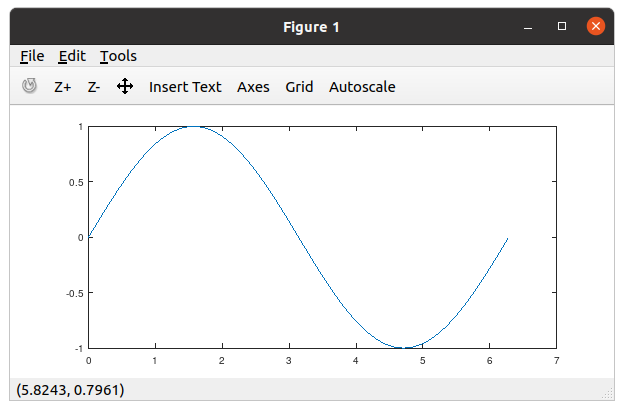
\includegraphics[width=0.4\textwidth]{imagem/senoX}
	\caption{Seno de X}
\end{figure}

A função \textit{plot(varX, varY)} gera gráficos lineares com os parâmetros \textbf{varX} variável independente e \textbf{varY} a dependente. Podemos adicionar mais séries plot(varX1, varY1, varX2, varY2) que gera dois gráficos combinados: \\
\codigo{>> plot([1, 1.5, 3], [5, 3, 5], [1, 2.5, 3], [5, 7, 5])}

Obtemos como resultado:
\begin{figure}[H]
	\centering
	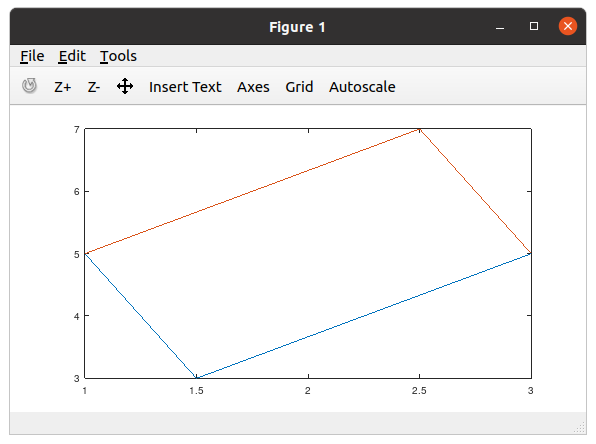
\includegraphics[width=0.4\textwidth]{imagem/grafico2}
	\caption{Gráficos combinados}
\end{figure}

Essas séries podem continuar indefinidamente. Vamos plotar o mesmo gráfico para senos (já visto anteriormente) com a adição do cosseno com algumas dessas opções: \\
\codigo{>> x = linspace(0, 2 * pi) \\
	>> plot(x, sin(x), 'r-', x, cos(x), 'b-') \\
	>> legend('Seno', 'Cosseno', 'location', 'southwest') \\
	>> title('Funções Seno e Cosseno de X') \\
	>> xlabel('Amplitude') \\
	>> ylabel('Frequência') \\
	>> grid on}

Obtemos como resultado:
\begin{figure}[H]
	\centering
	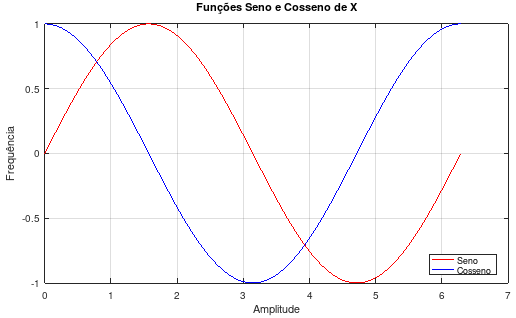
\includegraphics[width=0.6\textwidth]{imagem/senoEcosseno}
	\caption{Gráficos com Parâmetros}
\end{figure}

Foram colocados um terceiro parâmetro a cada série da função \textit{plot()} esses podem ser: \vspace{-1em}
\begin{itemize}[nolistsep]
	\item Cor: \textbf{y} (amarelo), \textbf{b} (azul), \textbf{c} (azul claro), \textbf{w} (branco), \textbf{r} (vermelho), \textbf{k} (preto), \textbf{m} (roxo) ou \textbf{g} (verde).
	\item Linha: \textbf{-} (sólida por padrão), \textbf{.} (pontos), \textbf{*}, \textbf{x}, \textbf{o} (diamantes) ou \textbf{v} (triângulos)
\end{itemize}

Para obtermos maiores informações sobre os parâmetros digitar \codigo{help axis}. Assim podemos dizer que esta função gráfica pode conter o seguinte: \textit{plot(serie1, serie2, ..., serieN)}. Sendo que cada série contém os valores de X, y e parâmetros.

\subsection{Barras e Histograma}
Barras e Histograma são gráficos bem comuns para quem trabalha de forma ativa com dados, o Octave também permite sua geração de um modo bem simples. Com a função \textit{bar()} temos um gráfico de barras: \\
\codigo{>> x = 1:10 \\
	>> y = randn(1, 10) \\
	>> bar(x, y)}

O vetor \textbf{x} é criado com valores de 1 a 10, e o vetor \textbf{y} utiliza a função \textit{randn(linha, coluna)} para gerar um vetor com 10 valores aleatórios. Obtemos como resultado:
\begin{figure}[H]
	\centering
	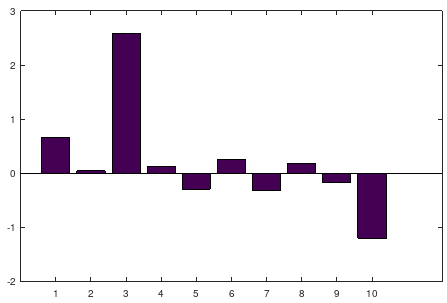
\includegraphics[width=0.5\textwidth]{imagem/barras}
	\caption{Gráfico de Barras}
\end{figure}

Como estamos com valores aleatórios o resultado pode variar. De mesmo modo podemos produzir um histograma, porém o primeiro valor passado é y (e não x) o segundo é número de bins. Podemos usar simplesmente: \\
\codigo{>> hist (randn(1, 100), 25)}

Obtemos como resultado provável:
\begin{figure}[H]
	\centering
	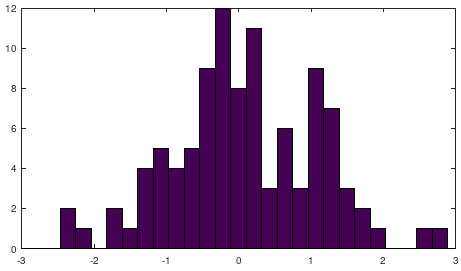
\includegraphics[width=0.5\textwidth]{imagem/histograma}
	\caption{Histograma}
\end{figure}

A função \textit{randn()} gera valores para uma distribuição normal. Podemos ainda utilizar as seguintes funções para gerarmos números aleatórios consistentes:
\begin{itemize}[nolistsep]
	\item \textit{discrete\_rnd(valor, probabilidade)}: distribuição discreta uni-variada.
	\item \textit{empirical\_rnd(dados)}: distribuição empírica.
	\item \textit{rande(n)}: distruição exponencial.
	\item \textit{randg(n)}: distribuição gama.
\end{itemize}	
	
Muitas vezes desejamos valores aleatórios inteiros, eles podem ser obtidos com a função \textit{randi()}, por exemplo: \\
\codigo{>> randi (10, 150, 1)}

Retorna 150 inteiros no range entre 1 e 10.

\subsection{Gráficos Tridimensionais}
A função \textit{mesh(varX, varY, varZ)} permite a projeção de gráficos tridimensionais: \\
\codigo{>> x = [0: 2 * pi / 50: 2 * pi]' \\
>> y = x \\
>> z = cos(x) * sin(y') \\
>> mesh(x, y, z)}

Cuidado para não esquecer de colocar o operador de transposição ($'$). Neste exemplo temos a função $z = cos(x) \times sin(y)$ no intervalo [0, 2pi] dividido em 50 incrementos. Obtemos como resultado:
\begin{figure}[H]
	\centering
	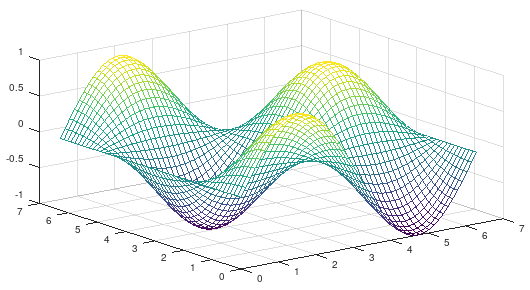
\includegraphics[width=0.5\textwidth]{imagem/graficoTri}
	\caption{Gráficos Tridimensional}
\end{figure}

\subsection{Coordenadas Polares}
A função \textit{polar(ângulo, r, 'parâmetros')} permite representar um ponto em coordenadas polares onde \textbf{r} é uma semi-reta com origem em ângulo (dados em radianos) e os parâmetros são combinações do tipo de linha e cor. Por exemplo: \\
\codigo{>> t = 0 : .01 : 2*pi \\
>> polar(t, sin(2*t).*cos(2*t), '-r')}

Obtemos como resultado:
\begin{figure}[H]
	\centering
	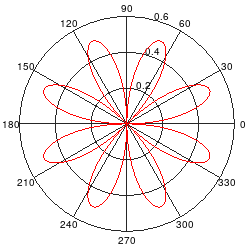
\includegraphics[width=0.35\textwidth]{imagem/polar}
	\caption{Cordenadas Polares}
\end{figure}

\section{Gráficos de Sequência discreta e Escada}
Esses tipos são apenas variações do gráfico de Barras, podemos obtê-los do seguinte modo: \\
\codigo{>> x = 0:0.5:4*pi \\
	>> y = sin(x) \\
	>> subplot(2,1,1) \\
	>> stem(x, y) \\
    >> subplot(2,1,2) \\
    >> stairs(x, y)}

Criamos com a função \textit{subplot(linha, coluna, indice)} uma área divisória para plotarmos o primeiro gráfico de sequência que é obtido com a função \textit{stem()}. Criamos uma segunda área para o segundo gráfico de escada que é dado pela função \textit{stairs()}. Obtemos como resultado:
\begin{figure}[H]
	\centering
	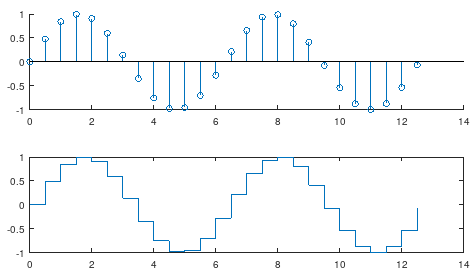
\includegraphics[width=0.6\textwidth]{imagem/sequenciaEscada}
	\caption{Gráficos de Sequencia e Escada na mesma figura}
\end{figure}

\section{Funções}
Podemos criar nossas funções personalizadas, fazemos isso para manter uma "biblioteca" de funções que mais necessitamos (como programas prontos para nosso uso). Vamos alternar da \opcmenu{Comand Window } para o \opcmenu{Editor } nas abas inferiores. Uma função tem a forma geral:
\begin{lstlisting}[]
function [saida] = nomeFuncao(parametros)
  comandos
endfunction
\end{lstlisting}

O arquivo deve ter o mesmo nome da função e possui a extensão ".m". Vamos criar a seguinte função:
\begin{lstlisting}[]
% somaProd
% Recebe dois parametros e calcula
% a soma e o produto entre os mesmos
function [soma, produto] = somaProd(a, b)
  soma = a + b;
  produto = a * b;
endfunction
\end{lstlisting}

É boa prática sempre documentarmos nossas funções, tudo o que estiver na frente do carácter de percentual é desprezado. Nossa função recebe dois valores \textbf{a} e \textbf{b}, retorna duas variáveis com a soma e o produto desses dois valores. Salvamos o arquivo com o nome "somaProd.m". Podemos usá-la  como se fosse uma função pré-existente no Octave. Alternar novamente para a \opcmenu{Comand Window}: \\
\codigo{>> [s, p] = somaProd(10, 3)}

A variável \textbf{s} recebeu a soma de 10 e 3 enquanto que \textbf{p} seu produto.

\subsection{Fluxos de Controle}
Nas funções são permitidos os seguintes fluxos de controle. Comando de decisão \textbf{if}:
\begin{lstlisting}[]
if condicao
  comandos caso verdadeiro
else 
  comandos caso falso 
endif
\end{lstlisting}

O laço de repetição determinada \textbf{for} do seguinte modo:
\begin{lstlisting}[]
for var = inicial:final
  comandos
endfor
\end{lstlisting}

Ou o laço de repetição indeterminada \textbf{while} do seguinte modo:
\begin{lstlisting}[]
while condicao
  comandos
endwhile
\end{lstlisting}

Caso seja necessário o comando \textbf{break} é utilizado para interromper as repetições do laço. Vejamos um exemplo com esses comandos:
\begin{lstlisting}[]
function [vetor] = ordenaVetor(vetor)
  troca = false
  while true
    for i = 1:length(vetor) - 1
      if vetor(i+1) < vetor(i)
        x = vetor(i+1)
        vetor(i+1) = vetor(i)
        vetor(i) = x
        troca = true
      endif
    endfor
    if !troca
      break
    else
      troca = false
    endif
  endwhile
endfunction

\end{lstlisting}

Como parâmetro recebemos um vetor para ordena-lo numericamente, criamos uma variável de controle para as trocas. Nosso laço indeterminado \textbf{while} (tem esse nome pois não sabemos quantas vezes seus comandos serão repetidos) será sempre repetido (em tese temos aqui um laço eterno). Entramos no laço determinado \textbf{for} (tem esse nome pois sabemos quantas vezes será executado do valor inicial da variável de entrada até o valor final) lemos da primeira posição do vetor (cuidado com outras linguagens pois aqui a primeira posição é 1) até sua última (dada pelo método \textit{lenght()}) menos 1 (pois usaremos para comparar a posição posterior). No comando de decisão \textbf{if} verificamos se a posição posterior é menor que a anterior em caso verdadeiro realizamos uma troca de valores e indicamos para a variável \textit{troca} que ocorreu. Ao término do laço \textbf{for} verificamos o conteúdo de \textbf{troca}, se for falso (ou seja nenhuma troca foi realizada) interrompemos o laço \textbf{while}, caso contrário voltamos o valor de \textbf{troca} para false e repetimos todo o processo.

Executamos essa função da seguinte maneira: \\
\codigo{>> x = ordenaVetor([4, 2, 5, 1])}

E como resultado teremos em \textbf{x} o valor ordenado: \\
\codigo{[1, 2, 4, 5]}

\section{Pacotes adicionais}
Por ser um software em constante desenvolvimento, vários outros pacotes adicionais podem ser instalados. Podemos ver uma lista completa desses em \url{https://octave.sourceforge.io/packages.php}. Antes de começarmos a instalar vamos verificar quais pacotes temos a disposição: \\
\codigo{>> pkg list}

Provavelmente a resposta será que não possuímos nenhum pacote instalado. Um boa biblioteca para instalarmos chama-se \textit{image}, localize e baixe o arquivo compactado (formato \textbf{tar.gz}). O editor está apontado para um determinado diretório de trabalho, o arquivo deve estar nesse diretório.
\begin{figure}[H]
	\centering
	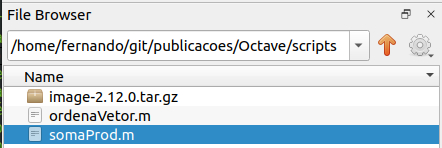
\includegraphics[width=0.5\textwidth]{imagem/diretorio}
	\caption{Diretório de Trabalho do Octave}
\end{figure}

Uma vez que temos isso acertado, instalamos com o comando: \\
\codigo{>> pkg install image-2.12.0.tar.gz}

\begin{theo}[No Ubuntu]{}
	Para o Ubuntu é necessário instalarmos o aplicativo \textit{liboctave-dev} para executarmos este comando. No terminal digite o comando: \codigo{\$ sudo apt install liboctave-dev}
\end{theo}

Com a conclusão da instalação, temos as seguintes funções a nossa disposição:
\begin{itemize}[nolistsep]
	\item $imread$: realizar a leitura da imagem.
	\item $image$: visualizar uma matriz como uma imagem.
	\item $imattributes$: atributos da imagem.
	\item $rgb2gray$: converter uma imagem colorida (RGB) em tons de cinza.
	\item $figure$: abrir uma nova janela gráfica.
	\item $colormap$: permitir a definição de um mapa de cores	
	\item $imfinfo$: retornar uma estrutura com diversas informações sobre a imagem.
\end{itemize}

Outras funções podem ser vistas consultando a documentação do pacote. Ao realizarmos a sua instalação esse já foi carregado, porém se sairmos e ao entrarmos novamente no Octave este não será reconhecido, é necessário carregá-lo com o comando: \\
\codigo{>> pkg load image}

Colocamos uma imagem no diretório de trabalho e a verificamos detalhes sobre ela: \\
\codigo{>> imfinfo("azaleia.jpg")}

Obviamente "azaleia.jpg" é o nome da imagem. Para carregá-la: \\
\codigo{>> azaleia = imread("azaleia.jpg");}

Observe o ";" ao término do comando isso fara suprimir a saída desse ou do contrário levará um bom tempo para ler. Os próximos comandos permitem visualizarmos a imagem: \\
\codigo{>> figure(1) \\
	>> image(azaleia)}

O primeiro abre a janela de visualização e o segundo mostra a imagem:
\begin{figure}[H]
	\centering
	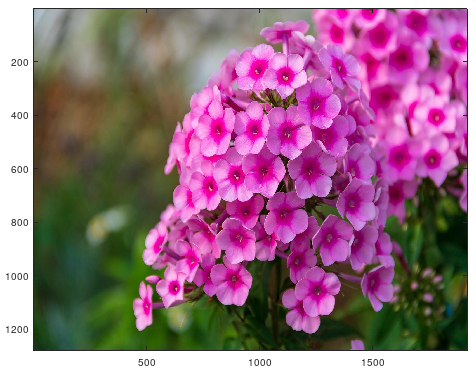
\includegraphics[width=0.3\textwidth]{imagem/azaleia}
	\caption{Imagem visualizada pelo Octave}
\end{figure}

Um erro muito comum de quem é iniciante ocorre quando convertemos a imagem para tons de cinza: \\
\codigo{>> azaleiag = rgb2gray(azaleia); \\
	>> figure(2) \\
	>> image(azaleiag)}

Obtemos como resultado:
\begin{figure}[H]
	\centering
	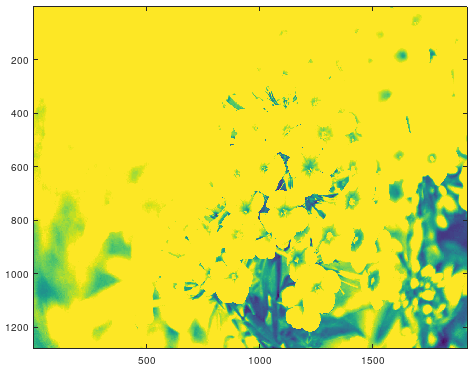
\includegraphics[width=0.3\textwidth]{imagem/azaleiag1}
	\caption{Imagem em tons de cinza}
\end{figure}

Precisamos "avisar" para o visualizador que agora deve trabalhar em tons de cinza não mais de modo colorido: \\
\codigo{>> colormap(gray(256))}

Obtemos como resultado:
\begin{figure}[H]
	\centering
	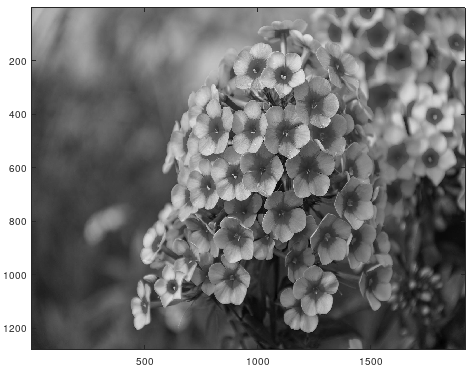
\includegraphics[width=0.3\textwidth]{imagem/azaleiag2}
	\caption{Imagem em tons de cinza correto}
\end{figure}

Podemos inclusive plotar a frequência e o tom de suas cores em um gráfico: \\
\codigo{>> figure(3) \\
	>> plot(hist(azaleiag(:), 0:255))}

E obtemos como resultado:
\begin{figure}[H]
	\centering
	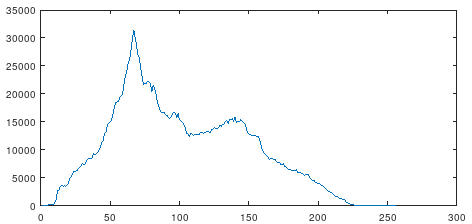
\includegraphics[width=0.6\textwidth]{imagem/azaleiHist}
	\caption{Histograma da Imagem}
\end{figure}

Outros pacotes bem interessantes para quem trabalha com tratamento de dados são: \vspace{-1em}
\begin{itemize}
	\item \textbf{Arduino}: que permite a comunicação com esta placa.
	\item \textbf{Database}: que provê acesso ao SGBD Postgres.
	\item \textbf{Dataframe}: que permite a criação de uma toolbox similar a do RStudio.
\end{itemize}

Sendo assim, não percamos a chance de explorá-los.

\section{Conclusão}
O GNU Octave é um aplicativo que foi originalmente desenvolvido com o propósito didático, mais especificamente para o projeto de reatores químicos e surgiu a partir da intenção de criar um aplicativo no qual a programação fosse mais rápida do que nas demais linguagens. Tornou-se é uma linguagem de alto nível, destinada principalmente a cálculos numéricos e estatísticos. Fornece uma completa interface utilizada para resolver problemas lineares e não-lineares ou executar outras experiências. Pode ser usado como uma linguagem base para executar roteiros complexos.

Sou um entusiasta do mundo \textbf{Open Source} e novas tecnologias. Qual a diferença entre Livre e Open Source? \underline{Livre} significa que esta apostila é gratuita e pode ser compartilhada a vontade. \underline{Open Source} além de livre todos os arquivos que permitem a geração desta (chamados de arquivos fontes) devem ser disponibilizados para que qualquer pessoa possa modificar ao seu prazer, gerar novas, complementar ou fazer o que quiser. Os fontes da apostila (que foi produzida com o LaTex) está disponibilizado no GitHub \cite{github}. Veja ainda outros artigos que publico sobre tecnologia através do meu Blog Oficial \cite{fernandoanselmo}.

%--------------------------------------------------------------------------
% REFERÊNCIAS
%--------------------------------------------------------------------------
\begin{thebibliography}{4}
	\bibitem{octaveoficial} 
	Página do Octave \\
	\url{https://www.gnu.org/software/octave/}
	
		\bibitem{fernandoanselmo} 
	Fernando Anselmo - Blog Oficial de Tecnologia \\
	\url{http://www.fernandoanselmo.blogspot.com.br/}
	
	\bibitem{publicacao} 
	Encontre essa e outras publicações em \\
	\url{https://cetrex.academia.edu/FernandoAnselmo}
	
	\bibitem{github} 
	Repositório para os fontes da apostila \\
	\url{https://github.com/fernandoans/publicacoes}
\end{thebibliography}

\end{document}